\documentclass[tikz,border=5pt]{standalone}
\usepackage[T1]{fontenc}
\usepackage{lmodern,amsmath,amssymb}
\usetikzlibrary{arrows.meta,calc,positioning,fit,backgrounds,shapes.geometric,matrix,decorations.pathreplacing,patterns}
\definecolor{ink}{gray}{0.08}
\definecolor{wash}{gray}{0.965}
\definecolor{soft}{gray}{0.45}
\tikzset{box/.style={draw=ink,line width=.65pt,fill=white,align=center,inner sep=4pt,outer sep=0pt,font=\small},flow/.style={draw=ink,line width=.65pt,-{Latex[length=1.8mm,width=1.3mm]},rounded corners=2pt},annotation/.style={font=\scriptsize,text=soft,align=center},groupbox/.style={draw=soft,dashed,line width=.45pt,fill=wash}}
\begin{document}
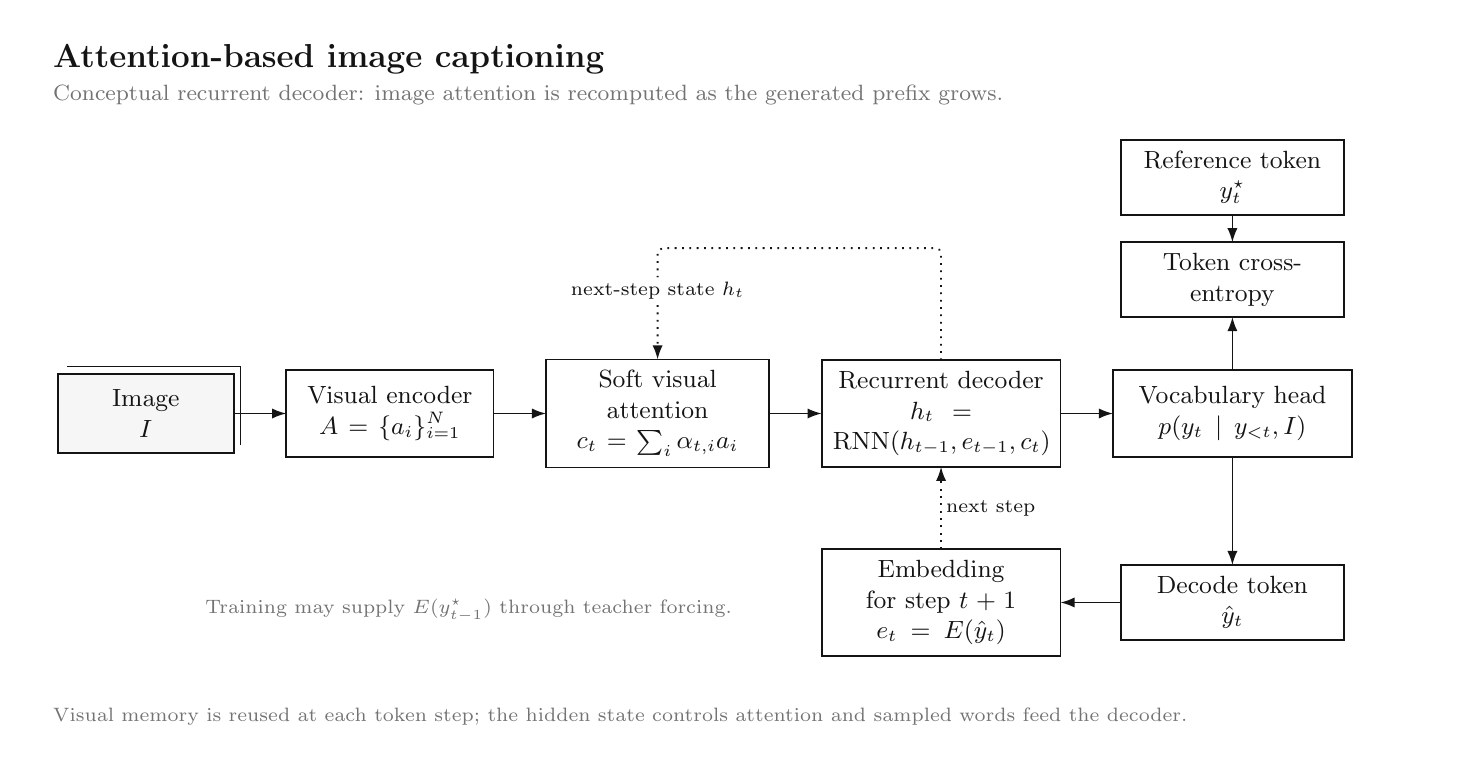
\begin{tikzpicture}[x=1cm,y=-1cm,font=\rmfamily,text=ink]

\path[use as bounding box] (0,0) rectangle (18,9);
\node[anchor=west,font=\large\bfseries] at (.2,.4) {Attention-based image captioning};
\node[anchor=west,font=\footnotesize,text=soft] at (.2,.85) {Conceptual recurrent decoder: image attention is recomputed as the generated prefix grows.};
\begin{pgfonlayer}{background}
\end{pgfonlayer}
\node[box,fill=wash,minimum width=2.2cm,minimum height=1cm,text width=1.9500000000000002cm] (image) at (1.5,4.9) {Image\\$I$};
\draw[ink,line width=.4pt] (0.4999999999999999,4.300000000000001) -- (2.7,4.300000000000001) -- (2.7,5.300000000000001);
\node[box,minimum width=2.6cm,minimum height=1.1cm,text width=2.35cm] (features) at (4.6,4.9) {Visual encoder\\$A=\{a_i\}_{i=1}^{N}$};
\node[box,minimum width=2.8cm,minimum height=1.1cm,text width=2.55cm] (att) at (8.0,4.9) {Soft visual attention\\$c_t=\sum_i\alpha_{t,i}a_i$};
\node[box,minimum width=3.0cm,minimum height=1.3cm,text width=2.75cm] (dec) at (11.6,4.9) {Recurrent decoder\\$h_t=\mathrm{RNN}(h_{t-1},e_{t-1},c_t)$};
\node[box,minimum width=3.0cm,minimum height=1.1cm,text width=2.75cm] (softmax) at (15.3,4.9) {Vocabulary head\\$p(y_t\mid y_{<t},I)$};
\node[box,minimum width=2.8cm,minimum height=0.9cm,text width=2.55cm] (target) at (15.3,1.9) {Reference token\\$y_t^{\star}$};
\node[box,minimum width=2.8cm,minimum height=0.8cm,text width=2.55cm] (loss) at (15.3,3.2) {Token cross-entropy};
\node[box,minimum width=2.8cm,minimum height=0.9cm,text width=2.55cm] (token) at (15.3,7.3) {Decode token\\$\hat y_t$};
\node[box,minimum width=3.0cm,minimum height=0.9cm,text width=2.75cm] (embed) at (11.6,7.3) {Embedding for step $t+1$\\$e_t=E(\hat y_t)$};
\begin{pgfonlayer}{background}
\draw[flow] (image.east) -- (features.west);
\draw[flow] (features.east) -- (att.west);
\draw[flow] (att.east) -- (dec.west);
\draw[flow] (dec.east) -- (softmax.west);
\draw[flow] (target.south) -- (loss.north);
\draw[flow] (softmax.north) -- (loss.south);
\draw[flow] (softmax.south) -- (token.north);
\draw[flow] (token.west) -- (embed.east);
\draw[flow,dotted] (embed.north) -- (dec.south) node[midway,right,fill=white,inner sep=1.5pt,font=\scriptsize] {next step};
\draw[flow,dotted] (dec.north) -- (11.6,2.8) -- (8.0,2.8) -- (att.north) node[midway,above,fill=white,inner sep=1.5pt,font=\scriptsize] {next-step state $h_t$};
\end{pgfonlayer}
\node[annotation,text width=7cm] at (5.6,7.4) {Training may supply $E(y_{t-1}^{\star})$ through teacher forcing.};
\node[anchor=west,align=left,font=\scriptsize,text=soft,text width=17.6cm] at (.2,8.75) {Visual memory is reused at each token step; the hidden state controls attention and sampled words feed the decoder.};
\end{tikzpicture}
\end{document}
